% This is a test for git, you can delete this particular line
% Note that the a4paper option is mainly intended so that authors in
% countries using A4 can easily print to A4 and see how their papers will
% look in print - the typesetting of the document will not typically be
% affected with changes in paper size (but the bottom and side margins will).
% Use the testflow package mentioned above to verify correct handling of
% both paper sizes by the user's LaTeX system.
%
% Also note that the "draftcls" or "draftclsnofoot", not "draft", option
% should be used if it is desired that the figures are to be displayed in
% draft mode.
%
%\documentclass[draftcls,onecolumn]{IEEEtran}
\documentclass[conference]{IEEEtran}
% Add the compsoc option for Computer Society conferences.
%
% If IEEEtran.cls has not been installed into the LaTeX system files,
% manually specify the path to it like:
% \documentclass[conference]{../sty/IEEEtran}


\usepackage{verbatim}
\usepackage{amstext}

\let\oldhat\hat
\renewcommand{\vec}[1]{\mathbf{#1}}
% \renewcommand{\hat}[1]{\oldhat{\mathbf{#1}}}


% Some very useful LaTeX packages include:
% (uncomment the ones you want to load)


% *** MISC UTILITY PACKAGES ***
%
%\usepackage{ifpdf}
% Heiko Oberdiek's ifpdf.sty is very useful if you need conditional
% compilation based on whether the output is pdf or dvi.
% usage:
% \ifpdf
%   % pdf code
% \else
%   % dvi code
% \fi
% The latest version of ifpdf.sty can be obtained from:
% http://www.ctan.org/tex-archive/macros/latex/contrib/oberdiek/
% Also, note that IEEEtran.cls V1.7 and later provides a builtin
% \ifCLASSINFOpdf conditional that works the same way.
% When switching from latex to pdflatex and vice-versa, the compiler may
% have to be run twice to clear warning/error messages.






% *** CITATION PACKAGES ***
%
%\usepackage{cite}
% cite.sty was written by Donald Arseneau
% V1.6 and later of IEEEtran pre-defines the format of the cite.sty package
% \cite{} output to follow that of IEEE. Loading the cite package will
% result in citation numbers being automatically sorted and properly
% "compressed/ranged". e.g., [1], [9], [2], [7], [5], [6] without using
% cite.sty will become [1], [2], [5]--[7], [9] using cite.sty. cite.sty's
% \cite will automatically add leading space, if needed. Use cite.sty's
% noadjust option (cite.sty V3.8 and later) if you want to turn this off.
% cite.sty is already installed on most LaTeX systems. Be sure and use
% version 4.0 (2003-05-27) and later if using hyperref.sty. cite.sty does
% not currently provide for hyperlinked citations.
% The latest version can be obtained at:
% http://www.ctan.org/tex-archive/macros/latex/contrib/cite/
% The documentation is contained in the cite.sty file itself.






% *** GRAPHICS RELATED PACKAGES ***
%
\ifCLASSINFOpdf
  \usepackage[pdftex]{graphicx}
  % declare the path(s) where your graphic files are
  % \graphicspath{{../pdf/}{../jpeg/}}
  % and their extensions so you won't have to specify these with
  % every instance of \includegraphics
  % \DeclareGraphicsExtensions{.pdf,.jpeg,.png}
\else
  % or other class option (dvipsone, dvipdf, if not using dvips). graphicx
  % will default to the driver specified in the system graphics.cfg if no
  % driver is specified.
  % \usepackage[dvips]{graphicx}
  % declare the path(s) where your graphic files are
  % \graphicspath{{../eps/}}
  % and their extensions so you won't have to specify these with
  % every instance of \includegraphics
  % \DeclareGraphicsExtensions{.eps}
\fi






% *** MATH PACKAGES ***
%
\usepackage[cmex10]{amsmath}
% A popular package from the American Mathematical Society that provides
% many useful and powerful commands for dealing with mathematics. If using
% it, be sure to load this package with the cmex10 option to ensure that
% only type 1 fonts will utilized at all point sizes. Without this option,
% it is possible that some math symbols, particularly those within
% footnotes, will be rendered in bitmap form which will result in a
% document that can not be IEEE Xplore compliant!
%
% Also, note that the amsmath package sets \interdisplaylinepenalty to 10000
% thus preventing page breaks from occurring within multiline equations. Use:
%\interdisplaylinepenalty=2500
% after loading amsmath to restore such page breaks as IEEEtran.cls normally
% does. amsmath.sty is already installed on most LaTeX systems. The latest
% version and documentation can be obtained at:
% http://www.ctan.org/tex-archive/macros/latex/required/amslatex/math/





% *** SPECIALIZED LIST PACKAGES ***
%
\usepackage{algorithmic}
% algorithmic.sty was written by Peter Williams and Rogerio Brito.
% This package provides an algorithmic environment fo describing algorithms.
% You can use the algorithmic environment in-text or within a figure
% environment to provide for a floating algorithm. Do NOT use the algorithm
% floating environment provided by algorithm.sty (by the same authors) or
% algorithm2e.sty (by Christophe Fiorio) as IEEE does not use dedicated
% algorithm float types and packages that provide these will not provide
% correct IEEE style captions. The latest version and documentation of
% algorithmic.sty can be obtained at:
% http://www.ctan.org/tex-archive/macros/latex/contrib/algorithms/
% There is also a support site at:
% http://algorithms.berlios.de/index.html
% Also of interest may be the (relatively newer and more customizable)
% algorithmicx.sty package by Szasz Janos:
% http://www.ctan.org/tex-archive/macros/latex/contrib/algorithmicx/




% *** ALIGNMENT PACKAGES ***
%
\usepackage{array}
% Frank Mittelbach's and David Carlisle's array.sty patches and improves
% the standard LaTeX2e array and tabular environments to provide better
% appearance and additional user controls. As the default LaTeX2e table
% generation code is lacking to the point of almost being broken with
% respect to the quality of the end results, all users are strongly
% advised to use an enhanced (at the very least that provided by array.sty)
% set of table tools. array.sty is already installed on most systems. The
% latest version and documentation can be obtained at:
% http://www.ctan.org/tex-archive/macros/latex/required/tools/


%\usepackage{mdwmath}
%\usepackage{mdwtab}
% Also highly recommended is Mark Wooding's extremely powerful MDW tools,
% especially mdwmath.sty and mdwtab.sty which are used to format equations
% and tables, respectively. The MDWtools set is already installed on most
% LaTeX systems. The lastest version and documentation is available at:
% http://www.ctan.org/tex-archive/macros/latex/contrib/mdwtools/


% IEEEtran contains the IEEEeqnarray family of commands that can be used to
% generate multiline equations as well as matrices, tables, etc., of high
% quality.


%\usepackage{eqparbox}
% Also of notable interest is Scott Pakin's eqparbox package for creating
% (automatically sized) equal width boxes - aka "natural width parboxes".
% Available at:
% http://www.ctan.org/tex-archive/macros/latex/contrib/eqparbox/





% *** SUBFIGURE PACKAGES ***
%\usepackage[tight,footnotesize]{subfigure}
% subfigure.sty was written by Steven Douglas Cochran. This package makes it
% easy to put subfigures in your figures. e.g., "Figure 1a and 1b". For IEEE
% work, it is a good idea to load it with the tight package option to reduce
% the amount of white space around the subfigures. subfigure.sty is already
% installed on most LaTeX systems. The latest version and documentation can
% be obtained at:
% http://www.ctan.org/tex-archive/obsolete/macros/latex/contrib/subfigure/
% subfigure.sty has been superceeded by subfig.sty.



%\usepackage[caption=false]{caption}
%\usepackage[font=footnotesize]{subfig}
% subfig.sty, also written by Steven Douglas Cochran, is the modern
% replacement for subfigure.sty. However, subfig.sty requires and
% automatically loads Axel Sommerfeldt's caption.sty which will override
% IEEEtran.cls handling of captions and this will result in nonIEEE style
% figure/table captions. To prevent this problem, be sure and preload
% caption.sty with its "caption=false" package option. This is will preserve
% IEEEtran.cls handing of captions. Version 1.3 (2005/06/28) and later 
% (recommended due to many improvements over 1.2) of subfig.sty supports
% the caption=false option directly:
\usepackage[caption=false,font=footnotesize]{subfig}
%
% The latest version and documentation can be obtained at:
% http://www.ctan.org/tex-archive/macros/latex/contrib/subfig/
% The latest version and documentation of caption.sty can be obtained at:
% http://www.ctan.org/tex-archive/macros/latex/contrib/caption/




% *** FLOAT PACKAGES ***
%
%\usepackage{fixltx2e}
% fixltx2e, the successor to the earlier fix2col.sty, was written by
% Frank Mittelbach and David Carlisle. This package corrects a few problems
% in the LaTeX2e kernel, the most notable of which is that in current
% LaTeX2e releases, the ordering of single and double column floats is not
% guaranteed to be preserved. Thus, an unpatched LaTeX2e can allow a
% single column figure to be placed prior to an earlier double column
% figure. The latest version and documentation can be found at:
% http://www.ctan.org/tex-archive/macros/latex/base/



\usepackage{stfloats}
% stfloats.sty was written by Sigitas Tolusis. This package gives LaTeX2e
% the ability to do double column floats at the bottom of the page as well
% as the top. (e.g., "\begin{figure*}[!b]" is not normally possible in
% LaTeX2e). It also provides a command:
\fnbelowfloat
% to enable the placement of footnotes below bottom floats (the standard
% LaTeX2e kernel puts them above bottom floats). This is an invasive package
% which rewrites many portions of the LaTeX2e float routines. It may not work
% with other packages that modify the LaTeX2e float routines. The latest
% version and documentation can be obtained at:
% http://www.ctan.org/tex-archive/macros/latex/contrib/sttools/
% Documentation is contained in the stfloats.sty comments as well as in the
% presfull.pdf file. Do not use the stfloats baselinefloat ability as IEEE
% does not allow \baselineskip to stretch. Authors submitting work to the
% IEEE should note that IEEE rarely uses double column equations and
% that authors should try to avoid such use. Do not be tempted to use the
% cuted.sty or midfloat.sty packages (also by Sigitas Tolusis) as IEEE does
% not format its papers in such ways.





% *** PDF, URL AND HYPERLINK PACKAGES ***
%
%\usepackage{url}
% url.sty was written by Donald Arseneau. It provides better support for
% handling and breaking URLs. url.sty is already installed on most LaTeX
% systems. The latest version can be obtained at:
% http://www.ctan.org/tex-archive/macros/latex/contrib/misc/
% Read the url.sty source comments for usage information. Basically,
% \url{my_url_here}.





% *** Do not adjust lengths that control margins, column widths, etc. ***
% *** Do not use packages that alter fonts (such as pslatex).         ***
% There should be no need to do such things with IEEEtran.cls V1.6 and later.
% (Unless specifically asked to do so by the journal or conference you plan
% to submit to, of course. )


% correct bad hyphenation here
\hyphenation{op-tical net-works semi-conduc-tor}


\begin{document}
%
% paper title
% can use linebreaks \\ within to get better formatting as desired
\title{Reliable power control for secondary users based on distributed measurements}


% author names and affiliations

% author names and affiliations
% use a multiple column layout for up to three different
% affiliations
%\author{\IEEEauthorblockN{Gitte Vanwinckelen \and Martijn Van Otterlo}
%\IEEEauthorblockA{Department of Computer Science\\
%Katholieke Universiteit Leuven\\
%Belgium\\
%Email: \{gitte\}.\{vanwinckelen\}@cs.kuleuven.be}
%\and
%\IEEEauthorblockN{Martijn Van Otterlo}
%\IEEEauthorblockA{Twentieth Century Fox\\
%Springfield, USA\\
%Email: homer@thesimpsons.com}
%\and
%\IEEEauthorblockN{James Kirk\\ and Montgomery Scott}
%\IEEEauthorblockA{Starfleet Academy\\
%San Francisco, California 96678-2391\\
%Telephone: (800) 555--1212\\
%Fax: (888) 555--1212}}

%\author{Gitte Vanwinckelen~$^{1}$ Martijn Van Otterlo~$^{1}$  Kurt Driessens~$^{2}$ Sofie Pollin~$^{3}$ \\
% \\
%$^1$ Katholieke Universiteit Leuven ~~ E-mail~:~ \{gitte\}.{\{vanwinckelen\}@cs.kuleuven.be}\\
%$^2$ Department of Knowledge Engineering ~~ E-mail~:~ \{gitte\}.{\{vanwinckelen\}@cs.kuleuven.be}\\
%$^3$ Interuniversity Micro-Electronics Center ~~E-mail~:~ pollins@imec.be \\}

\author{\IEEEauthorblockN{Gitte Vanwinckelen\IEEEauthorrefmark{1},  Martijn Van Otterlo\IEEEauthorrefmark{1},  Kurt Driessens\IEEEauthorrefmark{2} and  Sofie Pollin\IEEEauthorrefmark{3}}
\IEEEauthorblockA{\IEEEauthorrefmark{1}Department of Computer Science\\
Katholieke Universiteit Leuven, Belgium\\
Email:  gitte.vanwinckelen@cs.kuleuven.be, martijn.vanotterlo@cs.kuleuven.be}
\IEEEauthorblockA{\IEEEauthorrefmark{2}Department of Knowledge Engineering\\
Maastricht University, Netherlands\\
Email:  kurt.driessens@maastrichtuniversity.nl}
\IEEEauthorblockA{\IEEEauthorrefmark{3}Interuniversity Micro-Electronics Center \\
Leuven, Belgium\\
Email:  pollins@imec.be}
}


%\author{\IEEEauthorblockN{Gitte Vanwinckelen, Martijn Van Otterlo}
%\IEEEauthorblockA{Department of Computer Science\\
%Katholieke Universiteit Leuven\\
%Belgium\\
%Email:  gitte.vanwinckelen@cs.kuleuven.be \\
%martijn.vanotterlo@cs.kuleuven.be}
%\and
%\IEEEauthorblockN{Kurt Driessens}
%\IEEEauthorblockA{Department of Knowledge Engineering\\
%Maastricht University \\
%Netherlands\\
%Email:  kurt.driessens@maastrichtuniversity.nl}
%\and
%\IEEEauthorblockN{Sofie Pollin}
%\IEEEauthorblockA{Interuniversity Micro-Electronics Center,\\
%Leuven, Belgium\\
%Email:  pollins@imec.be}}

% conference papers do not typically use \thanks and this command
% is locked out in conference mode. If really needed, such as for
% the acknowledgment of grants, issue a \IEEEoverridecommandlockouts
% after \documentclass

% for over three affiliations, or if they all won't fit within the width
% of the page, use this alternative format:
% 
%\author{\IEEEauthorblockN{Michael Shell\IEEEauthorrefmark{1},
%Homer Simpson\IEEEauthorrefmark{2},
%James Kirk\IEEEauthorrefmark{3}, 
%Montgomery Scott\IEEEauthorrefmark{3} and
%Eldon Tyrell\IEEEauthorrefmark{4}}
%\IEEEauthorblockA{\IEEEauthorrefmark{1}School of Electrical and Computer Engineering\\
%Georgia Institute of Technology,
%Atlanta, Georgia 30332--0250\\ Email: see http://www.michaelshell.org/contact.html}
%\IEEEauthorblockA{\IEEEauthorrefmark{2}Twentieth Century Fox, Springfield, USA\\
%Email: homer@thesimpsons.com}
%\IEEEauthorblockA{\IEEEauthorrefmark{3}Starfleet Academy, San Francisco, California 96678-2391\\
%Telephone: (800) 555--1212, Fax: (888) 555--1212}
%\IEEEauthorblockA{\IEEEauthorrefmark{4}Tyrell Inc., 123 Replicant Street, Los Angeles, California 90210--4321}}




% use for special paper notices
%\IEEEspecialpapernotice{(Invited Paper)}




% make the title area
\maketitle


\begin{abstract}
%\boldmath
% Exact 200 woorden ! 
An important aspect of spectrum sharing is reliable protection of licensed, primary, users from interference by unlicensed, secondary, users. In this paper we investigate the reliability of the iterative power adjustment algorithm proposed by Pollin, Adams and Bahai (2008). The goal of this transmission power control algorithm is to allow a static secondary transmitter to maximize its power without interfering with primary users. A distributed flooding algorithm is used to detect primary users and estimate the distance to the primary propagation contour. The secondary transmitter makes a local channel estimation with a moving least squares algorithm to average out noise. The metric used to estimate interference is the propagation contour-contour distance between the secondary and primary transmitters. In our first contribution we investigate the reliability of this metric by computing the location probability, a new FCC proposed metric for configuring Digital Terrestrial Television networks. We show that the propagation contour-contour distance is correlated with the location probability. In a second contribution we make the flooding algorithm more cost efficient by reducing communication. We then study the influence of the number of flooding messages on the performance of the iterative power adjustment algorithm in terms of location probability and number of iterations.
\end{abstract}
% IEEEtran.cls defaults to using nonbold math in the Abstract.
% This preserves the distinction between vectors and scalars. However,
% if the conference you are submitting to favors bold math in the abstract,
% then you can use LaTeX's standard command \boldmath at the very start
% of the abstract to achieve this. Many IEEE journals/conferences frown on
% math in the abstract anyway.

% no keywords


% For peer review papers, you can put extra information on the cover
% page as needed:
% \ifCLASSOPTIONpeerreview
% \begin{center} \bfseries EDICS Category: 3-BBND \end{center}
% \fi
%
% For peerreview papers, this IEEEtran command inserts a page break and
% creates the second title. It will be ignored for other modes.
\IEEEpeerreviewmaketitle

Time, space and frequency spectrum are three important shared resources in wireless communications. But these resources are limited and with the continuous development of new wireless technologies and the increasing number of coexisting wireless networks there is a need to share these resources more efficiently. 
In this paper we focus on sharing space by transmission power control (TPC). In a wireless network we can make a distinction between \textit{primary} and \textit{secondary} users. Primary users are licensed and have priority to use the spectrum. Secondary users are not licensed and are only allowed to use the spectrum where it is not needed by the primary users and the interference that they cause to the primary users has to be minimized. In TPC, the goal is to make the transmission range of a secondary transmitter as large as possible while causing as little interference as possible to any primary users.

To find spectrum holes and compute its optimal transmission range, a secondary transmitter needs knowledge of the propagation conditions and the presence of primary users. In the literature three general approaches exist to find spectrum holes. The first approach is \textit{spectrum sensing} \cite{sensing1,sensing2}. A problem here are the high sensitivity requirements to detect all activity of the primary users and to overcome the hidden terminal problem. Studies conducted by both the Federal Communications Commission (FCC) and Electronic Communications Committee (ECC) have recently revealed serious doubts about the reliability of existing spectrum sensing solutions and have subsequently deferred from making these techniques an obligatory part of secondary use regulations. However, at the same time the FCC recognized the value of sensing for, for instance, the TV White Spaces in the following statement: ``We continue to believe that spectrum sensing will continue to develop and improve. We anticipate that some form of spectrum sensing may very well be included in TV Band Devices \cite{fcc}.''  In parallel to local sensing, other approaches are however needed to achieve a more reliable detection of spectrum. 

Instead of local sensing, \textit{cooperative} sensing can be used. Here the sensing results of multiple secondary users are combined to make a decision on the presence of a primary transmitter. A second approach to detect spectrum holes is \textit{geo-location} \cite{geoLocDyspan}. In this approach a user consults a central database to determine which frequencies are available at his location. A third approach is the use of dedicated signals, \textit{beacons}, to communicate the availability of frequencies \cite{beacon}.

In the work of Pollin, Adams and Bahai \cite{sofie}, an alternative approach to detect primary users is presented. A flooding algorithm is used to communicate the presence of primary transmitters to the rest of the network. This approach has some advantages. Like spectrum sensing, the approach is distributed and relies on field measurements. Therefore it does not require any additional infrastructure. Furthermore, responses to changes in the environment are quicker. Unlike spectrum sensing, no expensive high sensitivity sensing techniques are needed. 

In this \textit{iterative power adjustment} (IPA) algorithm, the power of the secondary transmitter is iteratively adapted based on the estimated distance between the interference threshold contours of the primary transmitters and the secondary transmitter. The estimated distance between the contours is communicated with a flooding algorithm from the primary transmitters throughout the rest of the network. The assumption is that the secondary transmitter causes no interference if a minimum distance between the contours of the primary transmitters and the contour of the secondary transmitter is respected.

Our first contribution is to investigate the reliability of the IPA algorithm by looking at the \textit{location probability}. In ECC report 159 \cite{ecc}, the location probability is defined as ``The probability with which a Digital Terrestrial Television (DTT) receiver would operate correctly at a specific location; i.e. the probability with which the median wanted signal level is appropriately greater than a minimum required value''.  According to the report, the location probability is widely used in the planning of DTT networks to measure the quality of coverage of a transmitter. Because the location probability takes into account interference from secondary transmitters, we can use it to test the reliability of the computation of the optimal transmission power by the IPA algorithm. We look at a scenario were the goal is reliable coexistence of a primary and a secondary DTT transmitter and show that there is a correlation between the location probability and the propagation contour-contour distance. 

In our second contribution we adapt the flooding step of the IPA algorithm to decrease the communication overhead. Besides the reduced overhead, this also implies a reduction of interference. We compare the performance of the original and the adapted IPA algorithm in terms of the number of iteration steps and the location probability. The algorithms are simulated in a two-dimensional environment that employs a general path loss model.

The paper is organized as follows. In Sec.~\ref{sec:pre} we give some preliminaries regarding the choice of the path loss model used in the simulations and the choice to use a flooding algorithm. Sec.~\ref{sec:ipa} then explains the IPA algorithm, which consists of three components: Received power estimation, distance-to-contour flooding and path loss estimation. Here, we also discuss the path loss model used in the simulations. In Sec.~\ref{sec:contri1} we study the reliability of the IPA algorithm in terms of the location probability. We relate the location probability to the propagation contour-contour distance metric used in the algorithm. Next, we propose the alternative distance-to-contour flooding algorithm and compare it with the original flooding algorithm in Sec.~\ref{sec:contri2}. We look at several performance metrics such as the number of forwarding users, location probability and number of iterations of the IPA algorithm. Conclusions are presented in Sec.~\ref{sec:conc}. 

%
\section{Preliminaries}\label{sec:pre}

The goal of the IPA algorithm is to find the optimal transmission power of any secondary transmitter. The optimal transmission power maximizes the transmission range of the secondary transmitter while causing no interference to any primary users. To find this power, a secondary transmitter needs knowledge of the radio propagation conditions and the presence of any primary transmitters. 
\subsection{Local power variance}

Radio propagation is typically modeled by a model consisting of three components: a distance dependent path loss trend, shadowing and fast fading. Shadow losses cause the received signal strength (RSS) to vary slowly in time and space around the distance dependent trend. Fast fading originates from multipath effects and causes the RSS to vary on a small scale \cite{bookPathlossModel}. Pollin, Adams and Bahai deduce from experiments that propagation conditions are difficult to model globally\footnote{In the measurement campaign of Pollin, Adams and Bahai \cite{sofie} the RSS from an 802.11 antenna on top of Cory Hall at UC Berkeley is measured in the area. They make three observations from the measurements. First, there is no obvious relationship between the RSS and the distance between the transmitter and the receiver. Second, the measurements show that shadowing is an anisotropic effect. Last, fast fading causes the RSS measurements to be noisy.}\cite{sofie}. Therefore, the IPA algorithm does not rely on a global propagation model but uses only local RSS measurements.

\subsection{Distance to contour flooding}
To detect the primary users and compute the distance between the transmission range of a primary user and the secondary user, no expensive sensing techniques are used. Instead, a more cost efficient distance-to-contour (DTC) flooding algorithm is used. This algorithm uses a back-off timer to decrease the number of forwarded messages with respect to regular flooding \cite{dtc}. With the DTC flooding algorithm, the number of forwarded messages is slightly larger than $n$, with $n$ being the number of users in the network. In this paper we develop an alternative distance-to-contour flooding algorithm which decreases the number of forwarded messages. This adapted flooding algorithm, DTC2, is based on the polygon tiling algorithm proposed by Hur et. al. \cite{dtc2}.

%%%%%%%%%%%%%%%%%%%%%%%%%%%%%%%%%%%%%%%%%%%%%%%%%%%%%%%%%%%%%%%%%%%%%%%%%%%%%%%%%%%%%%%%%%%%

\section{Iterative power adjustment algorithm}\label{sec:ipa}

\subsection{Overview}

We give an overview of the IPA algorithm in a situation with one primary and one secondary transmitter. However, the algorithm is also applicable in scenarios with multiple primary transmitters.
When the RSS of a user is used in the algorithm, an estimate $\hat{RSS}$ is computed with a MLS algorithm to average out the noise due to fast fading. This procedure is discussed in section \ref{sec:power est}.

First, receivers of the primary transmitters compute their $\hat{RSS}$ to find the users that define the interference threshold contour of the primary transmitter. Next, every user in the network is informed about his distance to the contour by means of the DTC flooding algorithm. DTC is discussed in section \ref{sec:dtc1}. Based on the distance to the contour of the primary transmitter and a worst case path loss model, a secondary transmitter can now make a first estimate of its transmission power. This initial estimate can iteratively be made more accurate based on information about the propagation conditions between the secondary and primary transmitter. First, the new contour-contour distance is taken into account. Second, the path loss between the contour of the secondary and primary transmitter is estimated at the user that is closest to the primary transmitter and still within the transmission range of the secondary transmitter. We discuss the iterative adaptation of the transmission power in section \ref{sec:pathloss est}.

\subsection{Local received power estimation} \label{sec:power est}

Reliable RSS estimates are needed for two reasons: To determine the interference threshold contours and to make accurate path loss estimations. The individual RSS measurements are noisy due to fast fading. In order to average out this noise, a MLS algorithm is used. This has the advantage that it does not rely on a global path loss model.

The MLS algorithm does not only take into account the RSS measurement of the user where the estimate is computed but also the measurements from the neighboring users. The size of the neighborhood is defined by a spatial weighting function (also called \textit{kernel function}). Assume we want to determine the $\hat{RSS}$ of user $N$ at position $x_N$. We search the coefficients $\vec{a}$ of a polynomial $\vec{p}$ by minimizing the weighted least squares function from equation \ref{eq:wls}. Polynomial $\vec{p}$ approximates the local RSS variations in the environment. To find $\vec{a}$, the local received power $RSS_N$ of user $N$ is taken into account together with the local received power $RSS_i$ of the neighbors of $N$, with $i=1..\#$Neighbors :
\begin{equation} \label{eq:wls}
\hat{\vec{a}}_N = \arg \min_a \sum_i w_{Ni}(\vec{a}^T \vec{p}(\vec{x}_i)-\vec{RSS_i})^2 \nonumber
\end{equation}
The local RSS measurements are weighted by $w_{Nj}$ according to the distance from user $N$, as demonstrated here:
\begin{equation} \label{eq:wij}
w_{Ni} = \begin{cases} 
(1-r_{Ni}^2)^3 &  \text{, if $r_{Ni} \leq 1$} \nonumber \\ 
0 & \text{, otherwise}
\end{cases}
\end{equation}
$r_{Ni}$ is the normalized distance between user $N$ and $i$. The distance is normalized by the kernel width $h$ as follows: $r_{Ni}=\frac{\begin{Vmatrix}\vec{x}_N-\vec{x}_i\end{Vmatrix}}{h}$.
From the coefficients $\hat{\vec{a}}_N$ we can compute $\hat{RSS}_N$ as:
\begin{equation}
\hat{RSS}_N = \hat{\vec{a}}^T_N \cdot \vec{p}(\vec{x}_N) \nonumber
\end{equation}

The MLS algorithm has two parameters: kernel width $h$ and the polynomial order of $\vec{p}$. These parameters depend on the noise power and can be optimized with respect to the average squared error on $\hat{RSS}$. This is demonstrated in the work of Pollin, Adams and Bahai \cite{sofie}. 

\subsection{Distance to contour flooding} \label{sec:dtc1}

An efficient flooding algorithm based on the algorithm proposed by Ye, Chen, Lu and Zhang \cite{dtc} is used to signal the presence of primary transmitters. The goal of the distance-to-contour flooding algorithm is to inform every user in the network about his distance to the contour of the primary user. A potential secondary transmitter can then determine the position of the wireless user within its transmission range that is closest to the contour of the primary user. In the next step of the IPA algorithm the path loss estimate of this closest secondary user is used to improve the estimate of the optimal transmission power of the secondary transmitter.

The centralized version of the DTC algorithm uses a priority queue to keep track of all information. Consider a scenario with transmitter P and $n$ wireless users. All users that receive P with a RSS larger than the interference contour threshold, $RSS_{th}$, are within the transmission range of P and are called \textit{internal} users. The \textit{footpoint} $f_i$ of a user $i$ with respect to P is defined as the internal user of P that is closest to $i$. The goal of the distance-to-contour algorithm is to inform all users about their footpoint $f$ and the distance $d$ to this footpoint.


\begin{enumerate}
\item During initialization all internal users of P are added to a priority queue. The footpoint of an internal user is the position of the user himself, $f_i = x_i$, and thus $d(i,f_i) = 0$. For all other users $d = \infty$.
\item The user with the smallest distance, user $N$, is taken from the queue. If more users share this smallest distance, one is randomly selected
\item User $N$ now informs his one-hop neighbors about his footpoint $f_N=x_A$. Based on this information the neighbors of $N$ update their footpoint and distance as follows: consider user $M$ which is a neighbor of $N$. The footpoint of $M$ is $f_M=x_B$ with $d(x_M,x_B)$. There are two possibilities:
\begin{enumerate}
 \item If $d(x_M,x_A) < d(x_M,x_B)$ then \\	
	$f_M \leftarrow x_A$ and $d(M,f_M) \leftarrow d(x_M,x_A)$ 
	, and $M$ is added to the queue.
 \item If $d(x_M,x_A) \geq d(x_M,x_B)$ then $f_M$ does not change and $M$ is not added to the queue.
\end{enumerate} 
 
\item When all the neighbors of $N$ are updated, $N$ is removed from the queue. The next user is now taken from the queue and all his neighbors are updated.
\item The process is repeated until the queue is empty
\end{enumerate}


To minimize the number of forwarding messages in the distance-to-contour flooding algorithm, the order in which users update their neighbors depends on their distance from P. In the centralized algorithm this is implemented by using a priority queue. In a practical scenario where users only communicate with their one-hop neighbors a priority queue cannot be used. The algorithm is made distributed by implementing the distance dependence with a back-off timer. 

Ideally, the time in which the network is updated equals $CW \cdot h$, with $h$ the communication range. The number of messages equals $n$, with $n$ the number of users in the network. In a practical scenario the update time and number of messages will be larger due to two reasons: 
 
\begin{itemize}
 \item Retransmissions are necessary because of collisions.
\item It is possible that a user starts updating his neighbors before he has obtained his closest footpoint. Wrong information is propagated to the neighbors and the user will have to update his neighbors a second time once he obtained his correct footpoint. We say the neighbors are \textit{misclassified}. This is illustrated in Fig.~\ref{fig:misclass}.
\end{itemize}

\begin{figure}
\centering
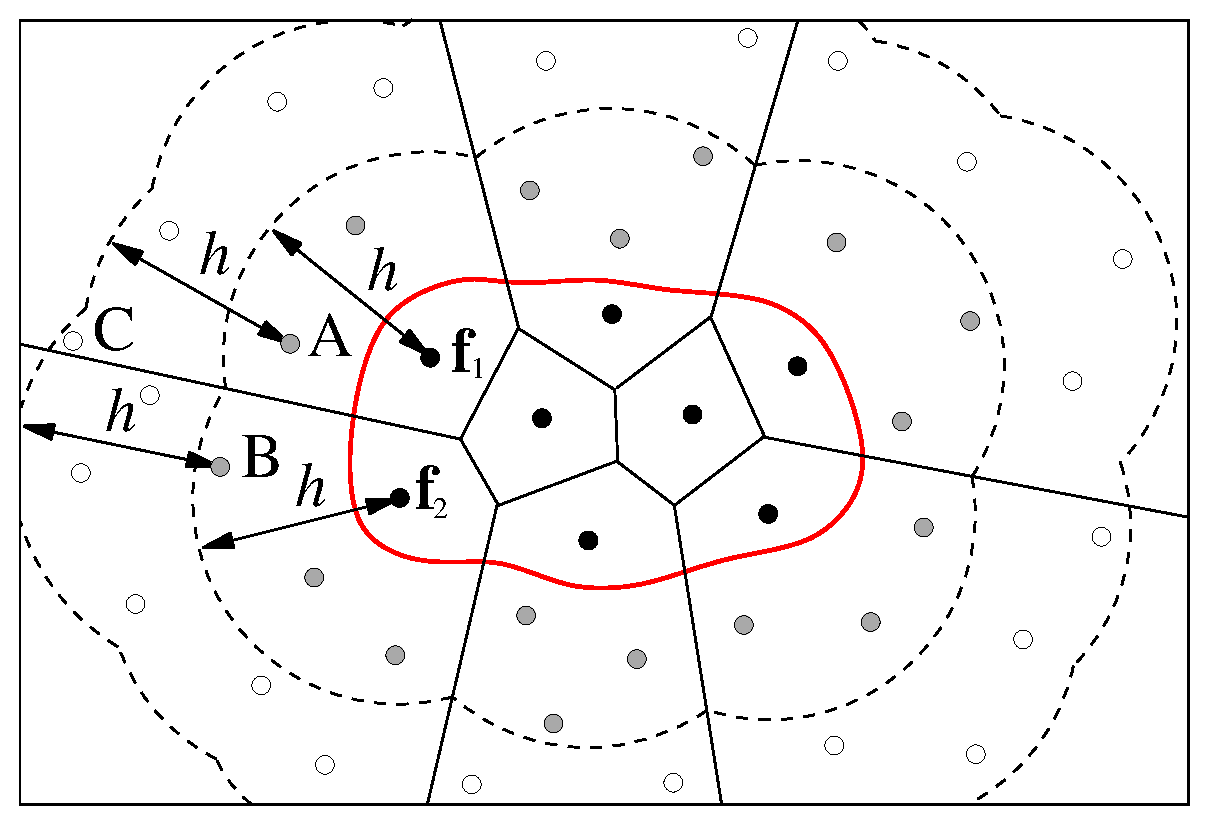
\includegraphics[scale=0.25]{figures/algorithm/proof2}
\caption{\label{fig:misclass}Users with the same footpoint are grouped together by a Voronoi Tiling. User C has footpoint $f_1$ and it lies in the transmission range of both users A and B. If the backoff timer of B goes off before the back-off timer of A, user C gets updated first by user B and it will incorrectly store $f_2$ as its footpoint. After user C is updated by user B, it starts a back-off timer to update its neighbors. However, when the back-off timer of user A goes off, C receives its correct footpoint $f_1$. If C has already updated its neighbors before it receives the update from A, user C will have to update its neighbors a second time. Figure from Pollin et.al. \cite{sofie} }
\end{figure}

\subsection{Path loss estimation} \label{sec:pathloss est}

When every user knows his distance to the contour of the primary transmitter P, a secondary transmitter S can estimate its optimal transmission power, $\hat{\textrm{power}}_S$, based on a local path loss estimate $\hat{PL}$ computed at the internal user of S that is closest to the primary contour, user $i_{cl}$. First, parameters $\alpha$ and $\beta$ of a path loss model are computed with a weighted least squares fit at $i_{cl}$. All the neighbors, $j$, within the kernel width $h$ around $i_{cl}$ are taken into account. This is shown in equation \ref{eq:fit}. Parameter $\alpha$ models the distance-dependent trend and $\beta$ consists of shadow and antenna losses. $d(S,j)$ is the distance between the transmitter S and a receiving user $j$. Next, the power of S is computed as the maximal interference power plus the estimated path loss between S and the contour of the primary transmitter. This is shown in equations \ref{eq:pow1} and \ref{eq:pow2}.
\begin{align}
&\hat{\alpha}_i,\hat{\beta}_i = \label{eq:fit} \\ \nonumber 
&\arg\min_{\alpha,\beta}\sum_j w_{ij}(\alpha10\log_{10} d(S,j)+\beta-\textrm{PL}_j)^2 \\
&\hat{\textrm{PL}}(S,f_{i_{cl}})=\hat{\alpha}10\log_{10}d(S,f_{i_{cl}})+\hat{\beta} \label{eq:pow1} \\
&\hat{\textrm{power}}_S=RSS_{th}+\hat{\textrm{PL}}(S,f_{i_{cl}}) \label{eq:pow2}
\end{align}

Note that it is hypothesized that the local path loss estimation at $i_{cl}$ gives information about the long range path loss between the primary and secondary transmitter. However, extrapolation over a long range and the presence of outliers can invalidate this hypothesis. We investigated a number of more complex approaches to solve this problem but they did not lead to a useful result. Further investigation is needed.

\subsection{Path loss model}

The IPA algorithm is tested in a simulated two-dimensional environment. In this section we present the path loss model used to simulate radio propagation conditions. The path loss $PL$ consists of four components which we discuss below: A distance dependent trend, antenna losses, shadowing and fast fading:
\begin{equation} \label{eq:plModel}
PL=10\alpha\log(d)+\gamma+L_S+X_{\sigma} \nonumber
\end{equation}
First, path loss increases exponentially with the distance $d$ from the transmitter. The rate of increase is modeled by parameter $\alpha$. Second, antenna losses are modeled by parameter $\gamma$. Third, shadow losses, $L_S$, are modeled by placing buildings in the scenario as explained in the work of Pollin, Adams and Bahai \cite{sofie}. Last, fast fading is modeled as Gaussian noise, $X_{\sigma}$, with variance $\sigma^2$. Pollin, Adams and Bahai showed that $\sigma^2=4$ is a realistic value for fast fading, thus this value is used in our simulations \cite{sofie}. However, the exact parameters of the path loss model are not important because the IPA algorithm only makes use of local path loss measurements.














% What is still missing in between sections? The pathloss model

\section{Reliability of the IPA algorithm in terms of location probability}\label{sec:contri1}

To determine the maximum transmission power of a secondary transmitter and ensure protection of the primary users, knowledge of the path propagation characteristics is needed. Examples of these characteristics are: the distances between the secondary transmitter and any primary transmitters, terrain shape and the relative antenna discrimination. The latter two characteristics determine the path loss $PL$. Although the characteristics are not known directly by the secondary transmitter, they can be estimated with the IPA algorithm. The distances between the secondary and primary transmitters can be computed with the distance-to-contour flooding algorithm and a local estimation of the path loss is computed with a MLS algorithm. In this section we investigate the reliability of the estimation of the path propagation characteristics by looking at the location probability.

\subsection[title]{Location probability$^2$}

\setcounter{footnote}{2}
\footnotetext{In this section we follow the description given in ECC report 159 \cite{ecc}.}

The location probability $q$ is defined as the probability with which a primary DTT receiver would operate correctly at a specific location, or gridpoint; i.e., the probability with which the median wanted signal level $P_P$ is appropriately greater then a minimum required value ;i.e.,
\begin{equation} \label{eq:lp}
q=Pr\{P_P\geq P_{P,min}+\sum_{i=1}^K r_{S,i}P_{S,i}\}=Pr\{P_P\geq S\} 
\end{equation}
In this formula, $P_{P,min}$ is the primary receiver's (noise-limited) reference sensitivity level \footnote{The reference sensitivity level of a receiver is the minimum wanted signal power for which the receiver can operate correctly in a noise-limited environment.}, $P_{S,i}$ is the received power of the $i^{th}$ unwanted, secondary, DTT signal and $r_{S,i}$ is the DTT-to-DTT protection ratio for the $i^{th}$ DTT transmitter; i.e., the minimum ratio of the wanted signal power and the interference signal power necessary for correct operation of the receiver. In the path loss model used in the simulations, the RSS at a gridpoint is a Gaussian variable were the mean $m$ is determined by the distance from the transmitter, antenna losses and shadowing. The variance $\sigma^2$ is determined by the amount of fast fading. Consider a gridpoint were a receiver senses the primary and secondary transmitter. We compute $Pr\{P_P\geq S\}$ at this gridpoint with Eq.~\ref{eq:lpCDF}.  as illustrated in Fig.~\ref{fig:compLP}. 


% Deze figuur zeker nog aanpassen!!! Letters kloppen niet en kwaliteit is niet ok!
\begin{figure}
\centering
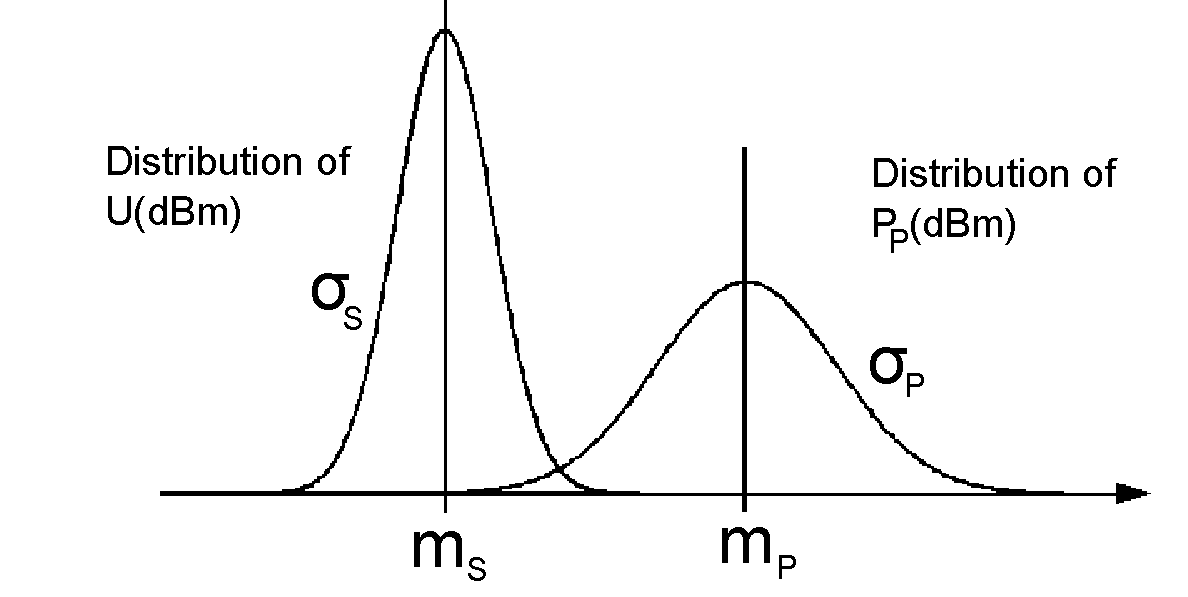
\includegraphics[scale=0.4]{figures/contribution1/distri.pdf}
\caption{\label{fig:compLP} \cite{ecc} The Gaussian distributions of the power of a secondary transmitter $S$ and a primary transmitter $P$ at one gridpoint. To compute the location probability at a location, we compute $Pr\{P_P\geq S\}$.}
\end{figure}

\begin{equation} \label{eq:lpCDF}
q=1-\frac{1}{2}\text{erfc}\{\frac{1}{\sqrt{2}}\frac{m_{S(dBm)}-m_{U(dBm)}}{\sqrt{\sigma_S^2+\sigma_U^2}}\}\
\end{equation}

\subsection{Simulation results}

A simulation of the IPA algorithm is shown in Fig.~\ref{fig:iterationsLP}. The effect of the secondary transmitter on the location probability of the primary transmitter for this simulation is illustrated by the results for example 2 in Tab.~\ref{tab:locProbEffect}. The table also shows the results for two other simulations.

\begin{table}
\caption{\label{tab:locProbEffect}Reliability of the IPA algorithm in terms of the location probability and overlap of the interference threshold contours for three different scenarios. }

\vspace{0mm}
\begin{tabular}{cccc}
\hline
          	&                 & $\Delta$ &	contour				\\
          	&                 & ($\%$)	& overlap ($\%$) PU	\\\hline
 example 1	& update 1				&	7				&	0							\\
 (2000 nodes)&update 2      	&	7				&	0							\\
            & update 3       	&	7.1			& 0							\\\hline 
 example 2	& update 1      	&	8				& 0							\\ 
 (1500 nodes)& update 2				& 9.1			& 0.3						\\\hline
            & update 1 				& 7.9			&	0							\\	
 example 2	& update 2 				& 7.9			&	0							\\	
 (1800 nodes)& update 3 			& 7.9			&	0							\\	
	          & update 4 				& 10.6			&	0							\\\hline		            

\end{tabular}
\vspace{-5mm}
\end{table}

\begin{figure}
\centering
\subfloat[primary transmitter]{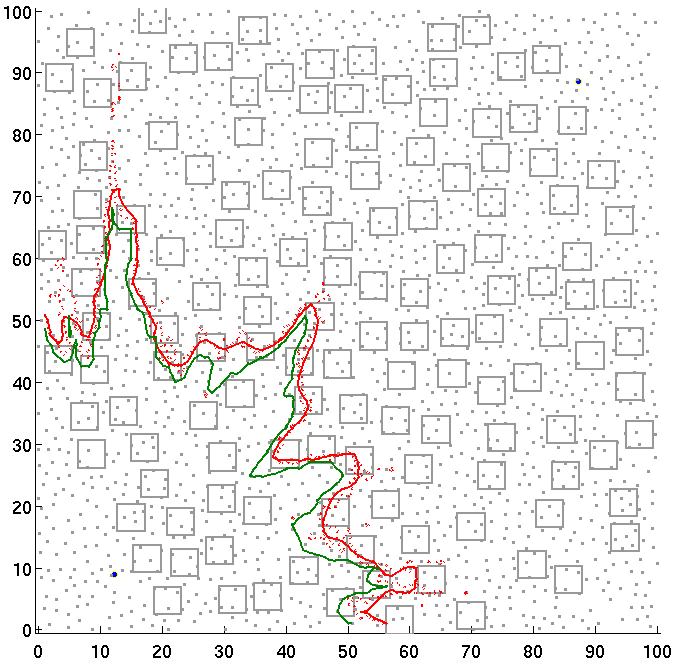
\includegraphics[scale=0.18]{figures/contribution1/vb2it0}} 
\subfloat[update 1]{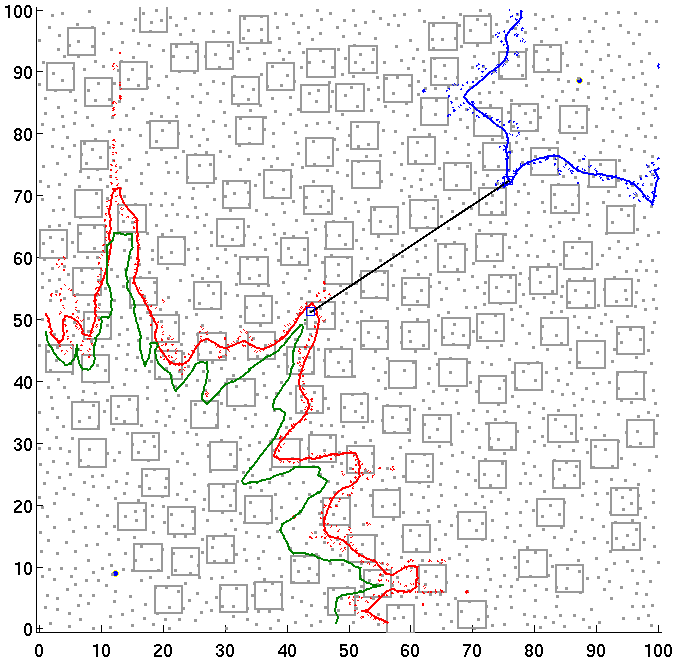
\includegraphics[scale=0.18]{figures/contribution1/vb2it1}} \\
\subfloat[update 2]{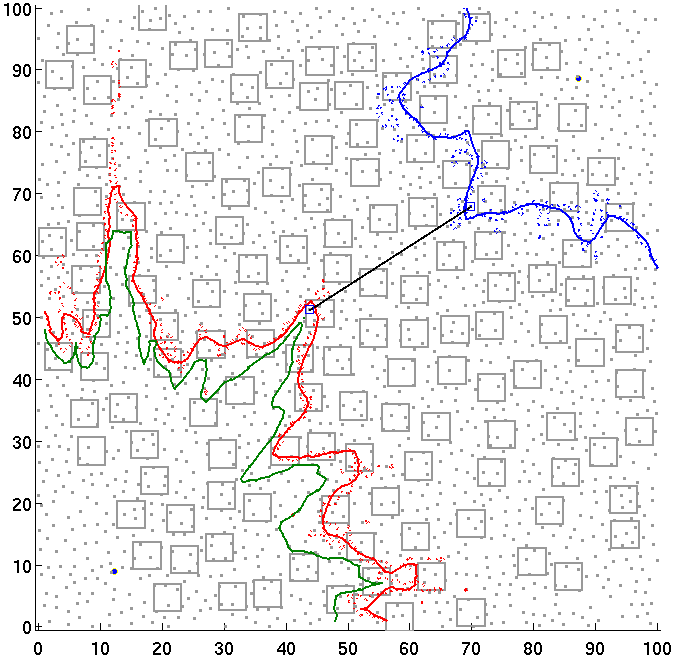
\includegraphics[scale=0.18]{figures/contribution1/vb2it2}}
\subfloat[update 3]{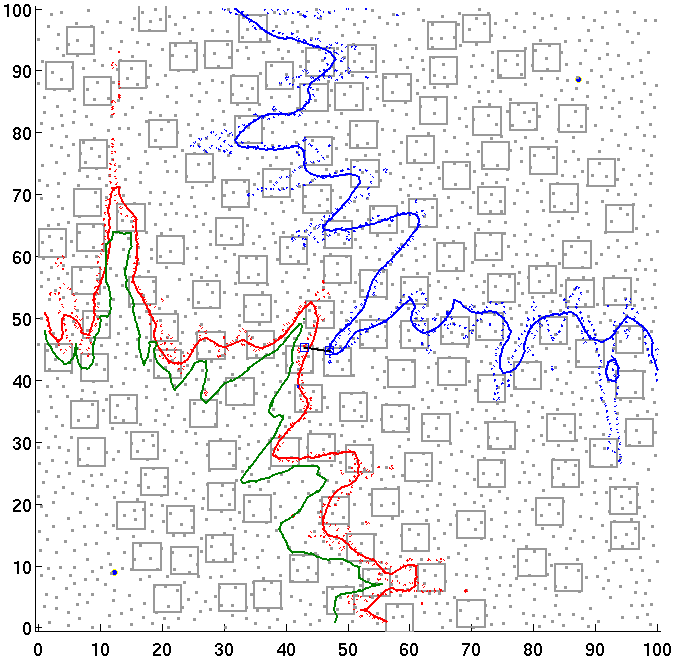
\includegraphics[scale=0.18]{figures/contribution1/vb2it3}}
\caption{\label{fig:iterationsLP} Demonstration of the IPA algorithm for example 2 from 
Tab.~\ref{tab:locProbEffect}. A primary transmitter is present in the lower left corner of the scenario and its interference threshold contour is indicated in red. The $95\%$ location probability contour is indicated in green. In the upper right corner a secondary transmitter is present with the interference contour indicated in blue.}
\end{figure}

In the second column of the table, $\Delta$ indicates the decrease of the area, $A$(textit{with SU}), of the $95\%$ location probability contour of the primary transmitter in comparison with the area of the contour when there is no interference from a secondary transmitter, $A$(\textit{no SU}), as shown in Eq.~\ref{eq:deltalp}. The decrease is indicated for every iteration of the IPA algorithm.

\begin{equation} \label{eq:deltalp}
\Delta=\frac{A(\textrm{\textit{no SU}})-A(\textrm{\textit{with SU}})}{A(\textrm{\textit{no SU}})}
\end{equation}

The third column shows the overlap of the interference threshold contours of the primary and the secondary transmitter as computed by the IPA algorithm. The overlap is expressed as the percentage of the area of the primary transmitter's contour that is overlapped by the contour of the secondary transmitter.

The simulations from Tab.~\ref{tab:locProbEffect} show that the presence of a secondary transmitter reduces the location probability with 7 to 10$\%$. The biggest reduction of the location probability is caused by the presence of a secondary transmitter and not by the increase in power as computed by the IPA algorithm. The reliability of the IPA algorithm is confirmed by Fig.~\ref{fig:connectionLPOverlap}. This figure shows that there is a relationship between the interference threshold contours computed by the IPA algorithm and the location probability. This justifies the use of the propagation contour-contour distance computed by the IPA algorithm as a metric for interference.

\begin{figure}
\centering
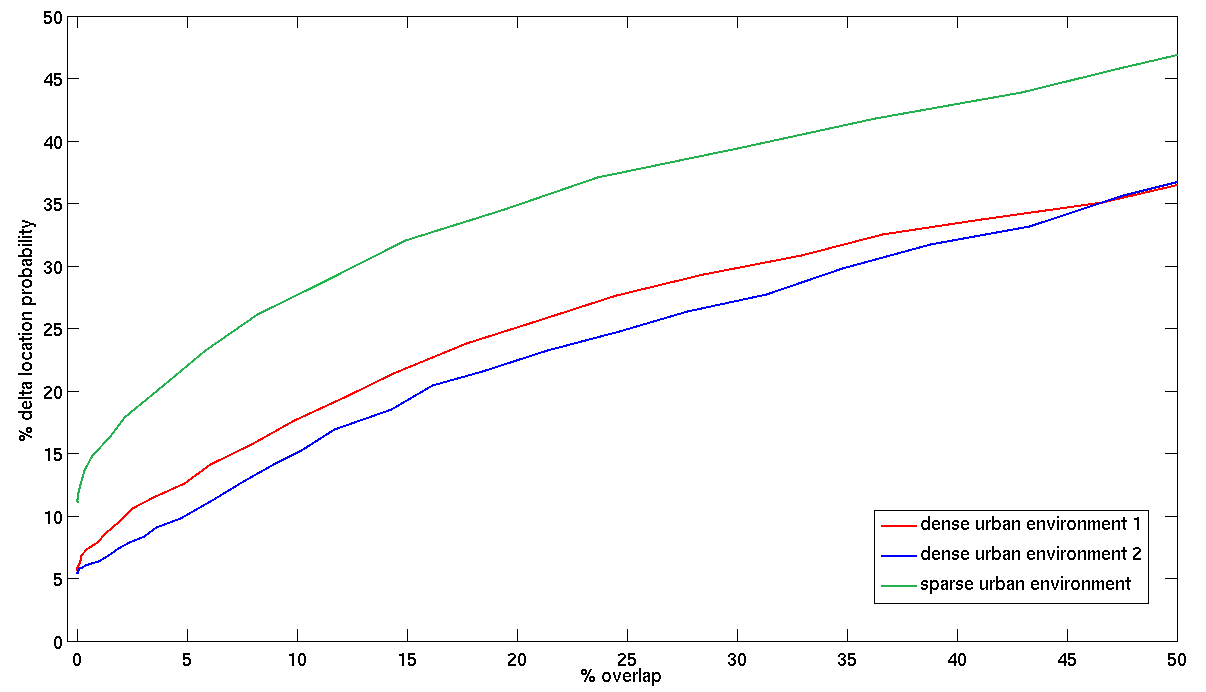
\includegraphics[scale=0.3]{figures/contribution1/correlation.png}
\caption{\label{fig:connectionLPOverlap} Reduction of the $95\%$ location probability contour in function of the overlap of the primary and secondary contour computed by the IPA algorithm.}
\end{figure}

% Remove table 2 since this tells the same story as the figure with the linear connection, it is a snapshot.
% \begin{table}
\caption{Performance of the algorithm for the examples of Fig.~\ref{fig:overlap}.
% the number
%of updates and the percentage of nodes misclassified for each contour propagation.
%Note that the number of updates to propagate the contour 
%is very close to $N$.
}
\vspace{0mm}
\begin{tabular}{ccc}
\hline
          	& 95$\%$ LP &	contour				\\
          	& $\Delta$	& overlap $\%$	\\\hline
 example 1	&	94.49			&	0							\\\hline 
 example 2	&	79.8			& 17.32					\\\hline        

\end{tabular}
\label{tab:overlap}\vspace{-5mm}
\end{table}


\begin{figure}
\centering
\subfloat[]{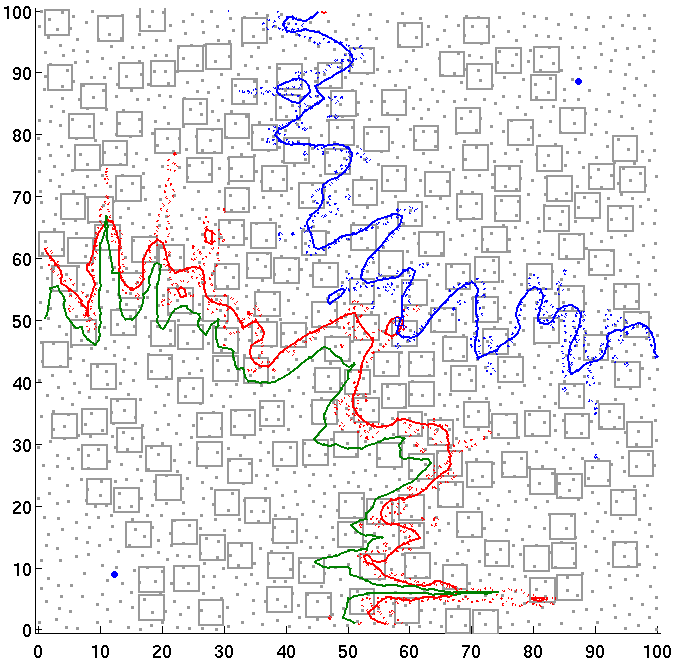
\includegraphics[scale=0.18]{figures/contribution1/vbNoOverlap}} 
\subfloat[]{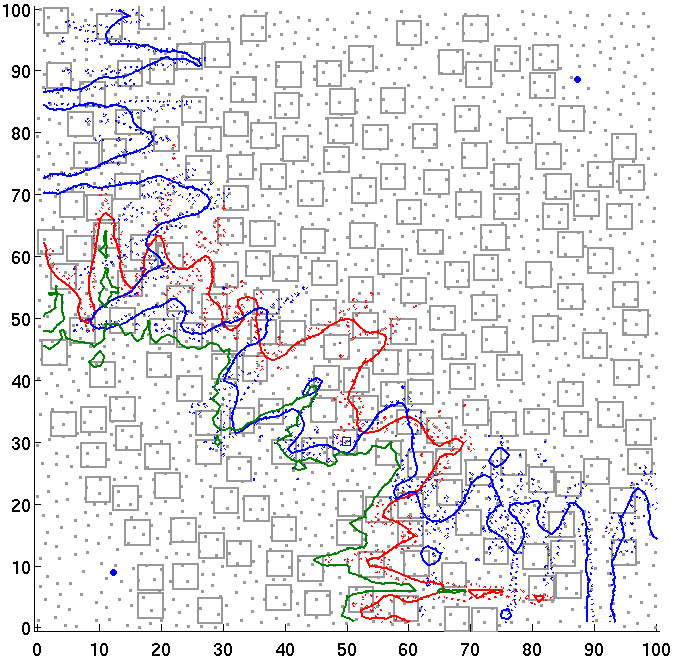
\includegraphics[scale=0.18]{figures/contribution1/vbOverlap}}
\caption{\label{fig:overlap} Demonstration of the effect of the overlap of the contours on the location probability. The results for this scenario are given in Tab.~\ref{tab:overlap} in terms of reduction of the location probability.}
\end{figure}




% Assumption which should also be mentioned in a preceding section: transmission range circular and of equal size.

\section{Redundancy reduction of distance-to-contour flooding}\label{sec:contri2}

Broadcasting information from a source user to the rest of the network with regular flooding causes problems such as redundancy, contention and collisions \cite{storm}. Redundant messages also unnecessarily increase the interference.  The distance-to-contour flooding algorithm reduces the number of flooding messages by using a back-off timer to impose an ordering on the transmitting users. For a network with $n$ users, the number of flooding messages is approximately equal to $n$. In this section we propose an alternative to DTC that reduces the number of transmitting users further. From now on, we refer to the adapted distance-to-contour flooding algorithm as the DTC2 flooding algorithm. 

Flooding algorithms can be divided into three categories based on the amount of information users needs from their neighbors \cite{1hopflooding}. The first category are the flooding algorithms that require no information, for example \textit{regular} flooding and \textit{probabilistic} flooding. Algorithms from the second category reduce redundant transmissions by having every user select only a subset of its neighbors to forward a message. For this, a user needs information about his \textit{one-hop} (direct) neighbors. DTC2 belongs to this category. Another example can be found in the work of Liu, Jia Wan et.al. \cite{1hopflooding}. The third category contains algorithms that use information about neighbors that are \textit{two hops} or more away \cite{2hop}. 

\subsection{Ideal network topology}

DTC2 selects the forwarding neighbors according to the selection criterium proposed by Hur, Duc Le and Choo \cite{dtc2}. The idea is to approximate an ideal network topology where the overlapping area of the users' transmission ranges is minimized. Fig.~\ref{fig:threeforwards} and Fig.~\ref{fig:fourforwards} show the ideal topology for a user with respectively three and four neighbors and Fig.~\ref{fig:hextiling} and Fig.~\ref{fig:squaretiling} show the resulting hexagonal and square tiling topology in a network. We chose to investigate the square tiling topology from Fig.~\ref{fig:fourforwards} because there is less redundancy in the communication when a user only forwards to four neighbors instead of six neighbors in the hexagonal tiling topology.

In a real network the users are deployed randomly and previous discussed topologies do not occur, so the criterium to select forwarding neighbors is to choose the neighbors located closest to the ideal positions. By reducing the number of forwarding neighbors, the number of transmissions and collisions is also reduced. By choosing the users closest to the ideal positions we aim to have all users in the network receive updates. We express this in terms of the \textit{delivery ratio}, which is the ratio of the number of users that receive flooding messages to the total number of users in the network.

\begin{figure}
\centering
\subfloat[]{\label{fig:threeforwards}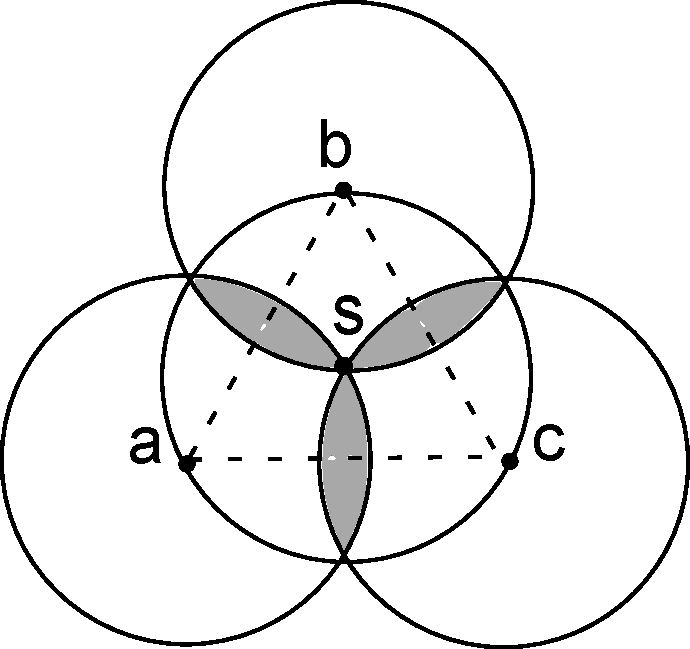
\includegraphics[scale=0.25]{figures/contribution2/threeForwarding.pdf}} \hspace{8mm}
\subfloat[]{\label{fig:fourforwards}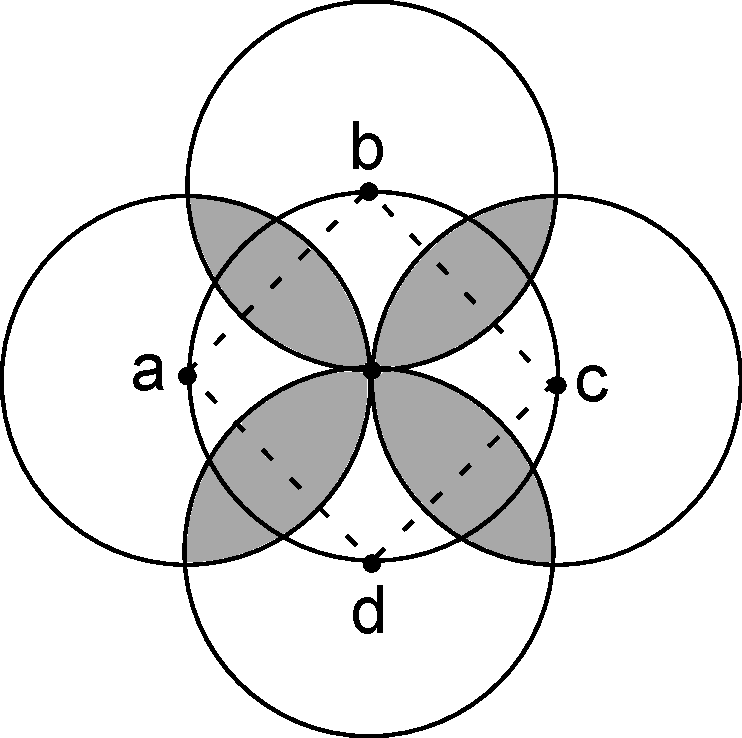
\includegraphics[scale=0.26]{figures/contribution2/fourForwarding.pdf}}  \\ \hspace{3mm}
\subfloat[]{\label{fig:hextiling}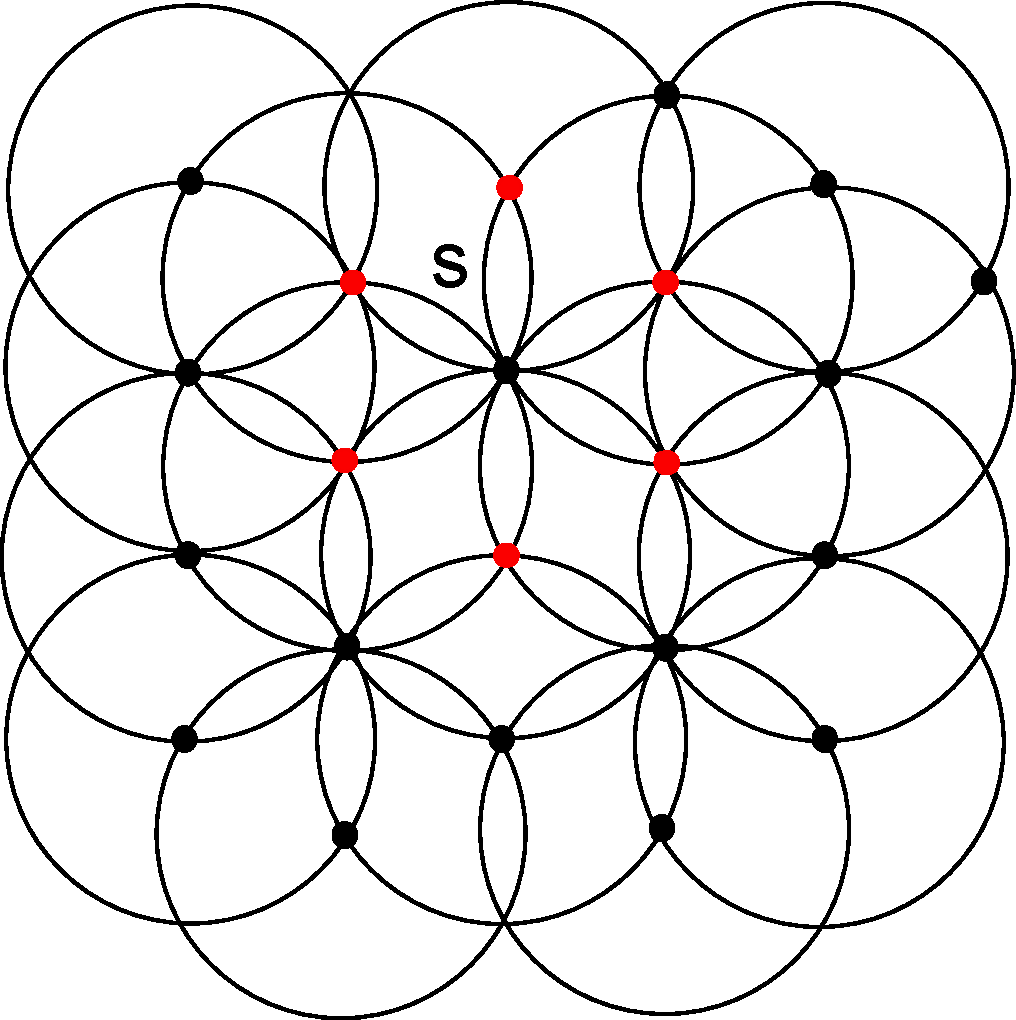
\includegraphics[scale=0.17]{figures/contribution2/hexagonalTiling.pdf}} \hspace{8mm}
\subfloat[]{\label{fig:squaretiling}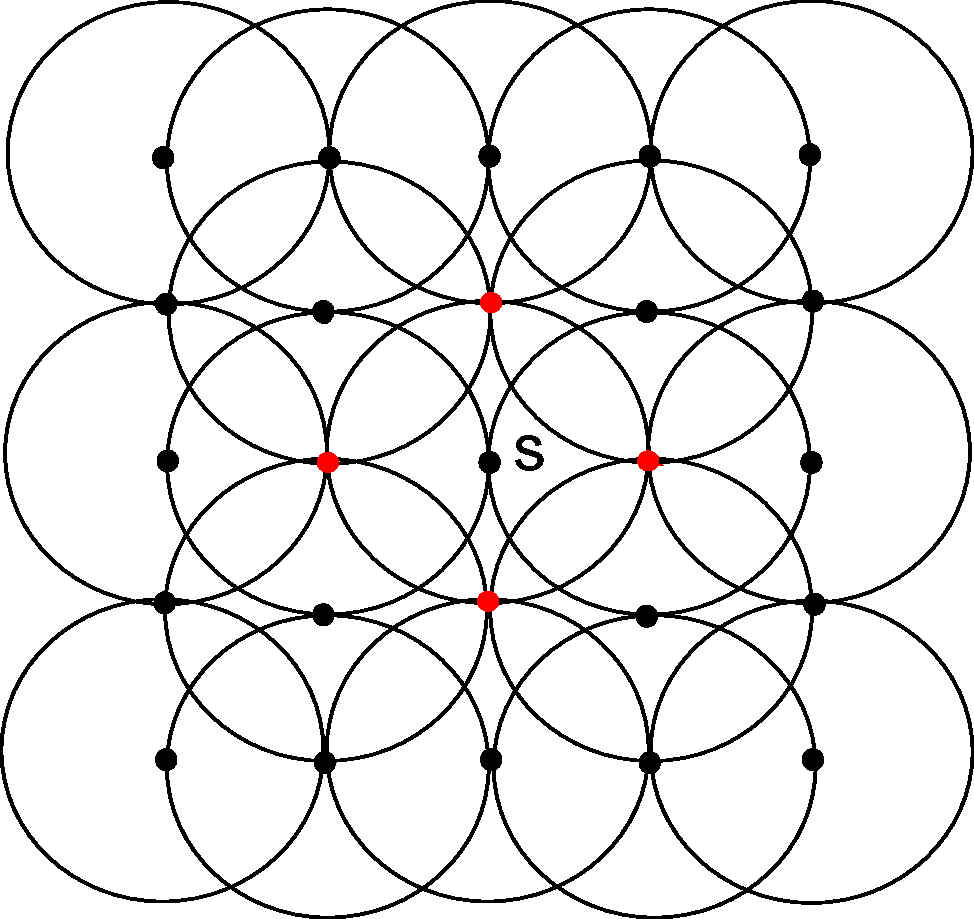
\includegraphics[scale=0.21]{figures/contribution2/squareTiling.pdf}}
\caption{\label{fig:forwarding} \cite{dtc2} Fig.~\ref{fig:threeforwards} and Fig.~\ref{fig:fourforwards} show the ideal topology for a user with respectively three and four neighbors. This topology minimizes the overlapping areas of the transmission ranges. Fig.~\ref{fig:hextiling} and Fig.~\ref{fig:squaretiling} show the resulting network topologies for respectively three and four neighbors.}
\end{figure}
% Square tiling is zeer vreemd, check dit nog eens !!!! extra cirkel overal toevoegen in b en d , lost probleem op

\subsection{Forwarding user selection}\label{subsec:forwardingSel}

The procedure to select forwarding neighbors is described by Hur, Duc Le and Choo as follows:

We assume every user knows his position by GPS or a positioning algorithm. Consider user $s$ from Fig.~\ref{fig:partitioning} with co\"ordinates $(x_S,y_S)$. Partitions $P_0,P_1,P_2$ and $P_3$ divide the transmission range of $s$ in four as illustrated in Fig.~\ref{fig:partitioning1}. 

\begin{figure}
\centering
\subfloat[]{\label{fig:partitioning1}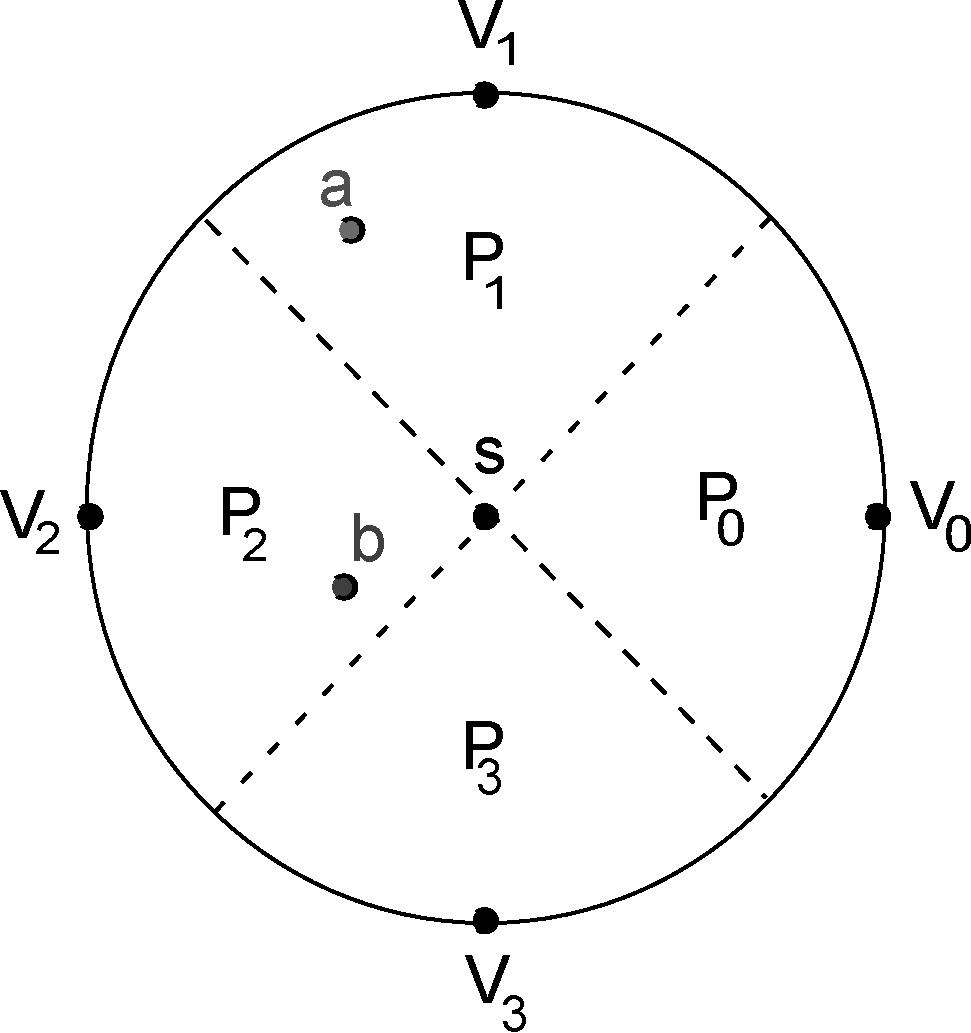
\includegraphics[scale=0.2]{figures/contribution2/partitioning.pdf}} \hspace{6mm}
\subfloat[]{\label{fig:partitioning2}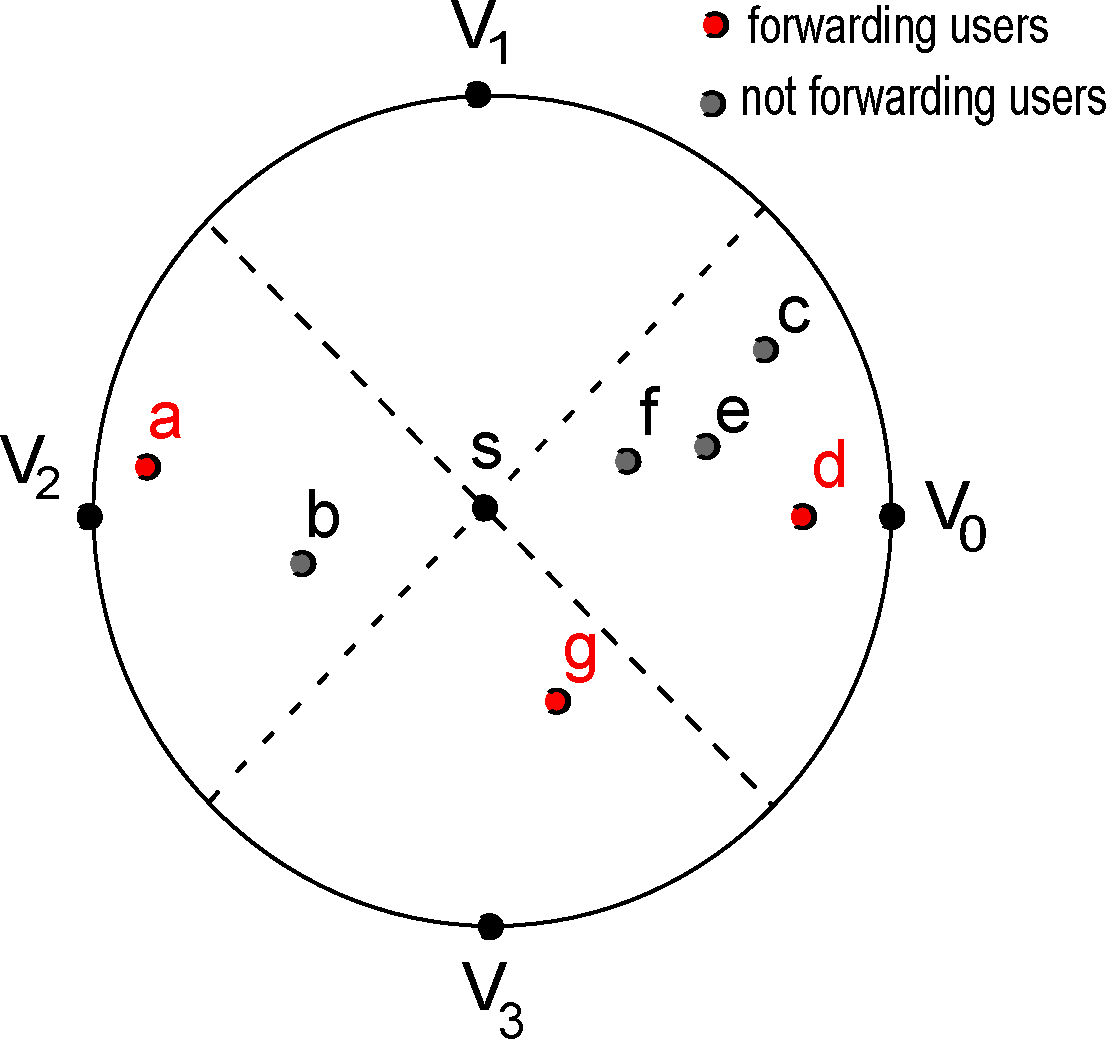
\includegraphics[scale=0.2]{figures/contribution2/userSelection.pdf}}
\caption{\label{fig:partitioning}\cite{dtc2}   Fig.~\ref{fig:partitioning1} demonstrates the partitioning of the transmission range of user $s$. Fig.~\ref{fig:partitioning2} shows an example of which users are selected as forwarding neighbors. }
\end{figure}

With every partition $P_i$ there is one vertex $V_i$ associated, with $0\leq i\leq3$. These vertices indicate the positions of the four forwarding neighbors in case of an ideal square tiling topology. A user determines the forwarding neighbors as follows: For each partition $P_i$ the neighbor closest to $V_i$ is selected. If the partition is empty, no neighbor is selected. The selection is illustrated in Fig.~\ref{fig:partitioning2}.

Where in step three of the DTC algorithm, all the neighbors of a user forward their footpoint, in DTC2 only a subset of forwarding neighbors is selected. We consider again a scenario with transmitter P and $n$ wireless users and describe this third step of DTC2 in which a user $N$ updates his one-hop neighbors about his footpoint $f_N=x_A$. Based on this information the neighbors of $N$ update their footpoint and distance in the same way as in the DTC flooding algorithm. user $N$ also computes the set of forwarding neighbors $F(N)$ as discussed above. 

Consider the following example of the update and forwarding process for a neighbor of user $M$ that is a neighbor of user $N$. User $N$ has footpoint $f_N=x_A$ and distance $d(x_N,x_A)$ to this footpoint. User $M$ has footpoint $f_M=x_B$ and distance $d(x_M,x_B)$ to this footpoint. There are two possibilities:

\begin{enumerate}
\item If $d(x_M,x_A) < d(x_M,x_B)$, then $f_j \leftarrow x_A$ and $d(x_M,f_M) \leftarrow d(x_M,x_B)$. 
	\begin{itemize}
	\item If user $M \not\in F(N)$, $M$ is not added to the queue.
	\item Otherwise, $M$ is added to the queue.
	\end{itemize}
\item If $d(x_M,x_A) \geq d(x_M,x_B)$, then the footpoint of $M$ does not change and user $M$ is not added to the queue, independent of whether it is a member of $F(N)$.
\end{enumerate}
 
\subsection{Simulation results}


\begin{figure*}[!b]
\centering 
\subfloat[]{\label{fig:dtc2nbSends}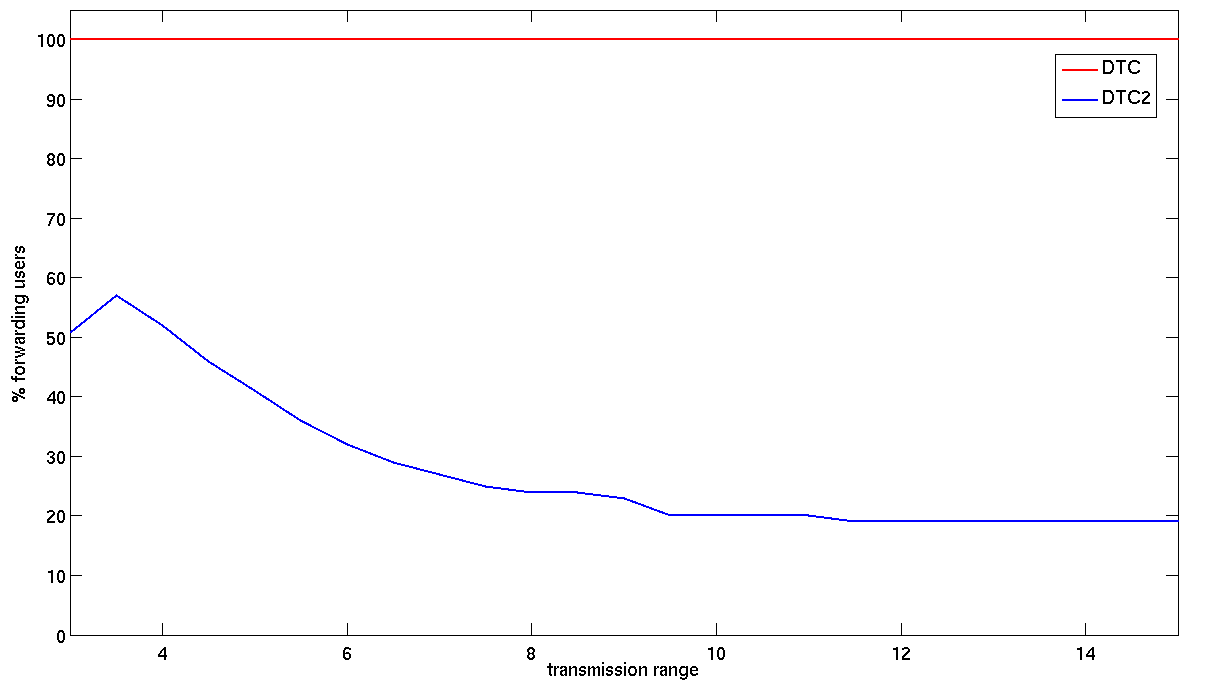
\includegraphics[scale=0.16]{figures/contribution2/nbSends2}} \hspace{1cm}
\subfloat[]{\label{fig:dtc2locprob}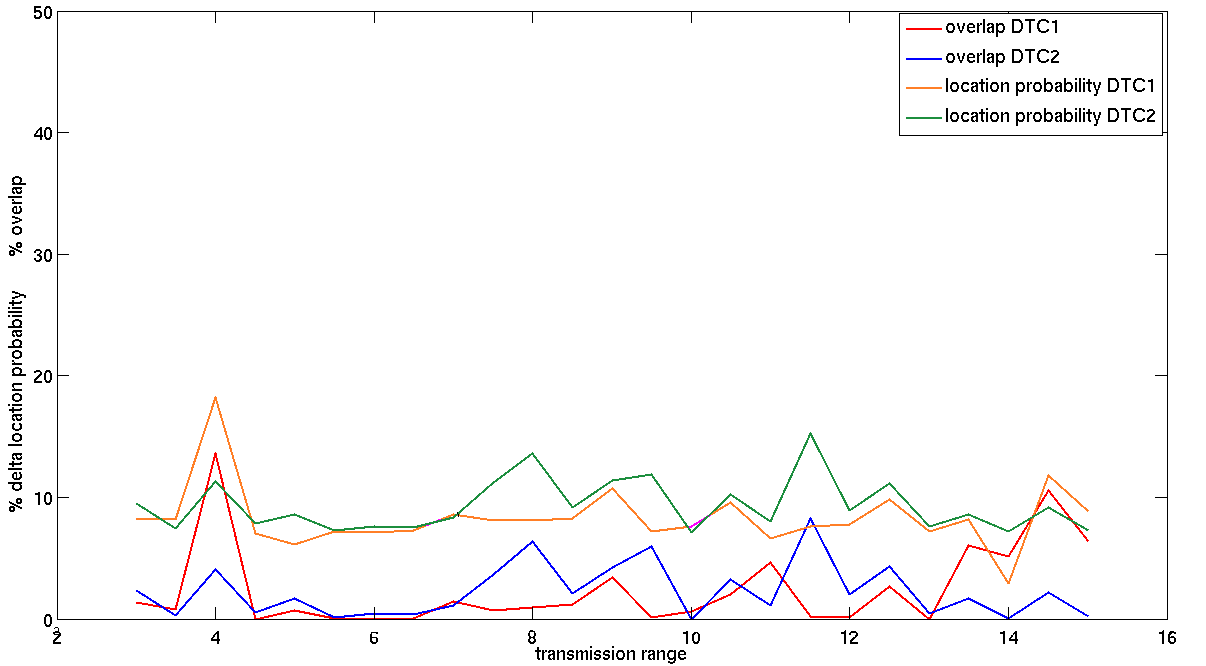
\includegraphics[scale=0.27]{figures/contribution2/locproboverlap2}} \\
\subfloat[]{\label{fig:dtc2misclass}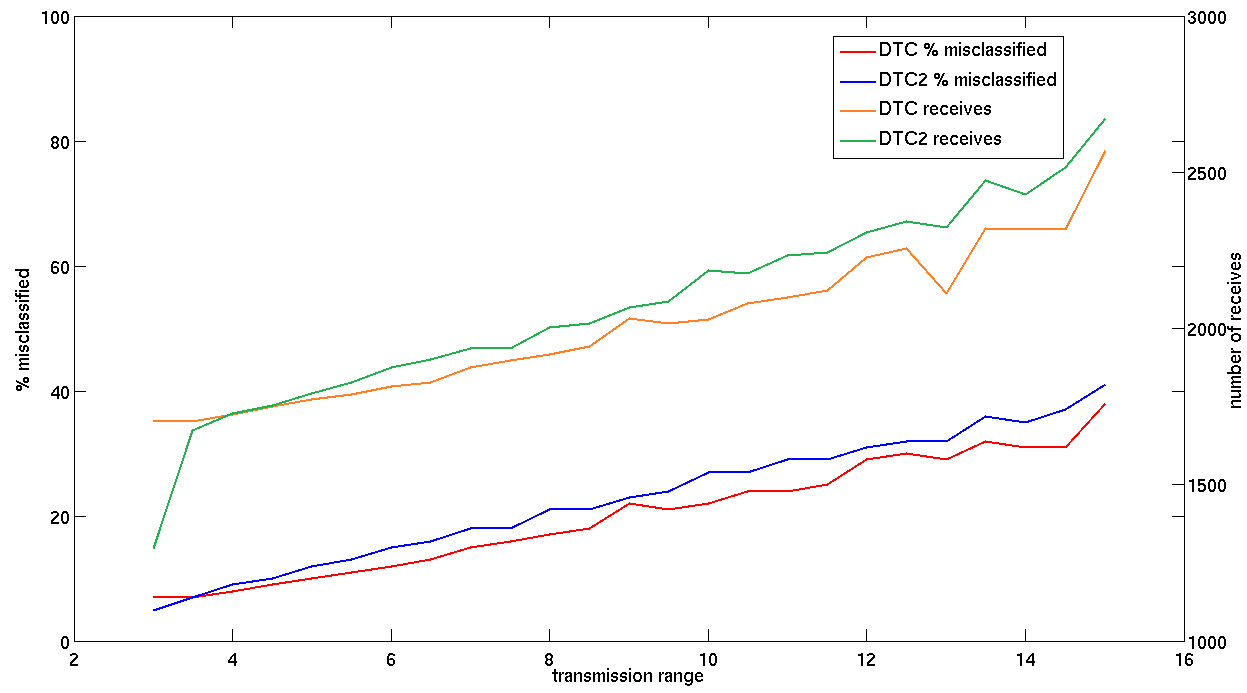
\includegraphics[scale=0.26]{figures/contribution2/misclassified2}}\hspace{1cm}
\subfloat[]{\label{fig:dtc2error}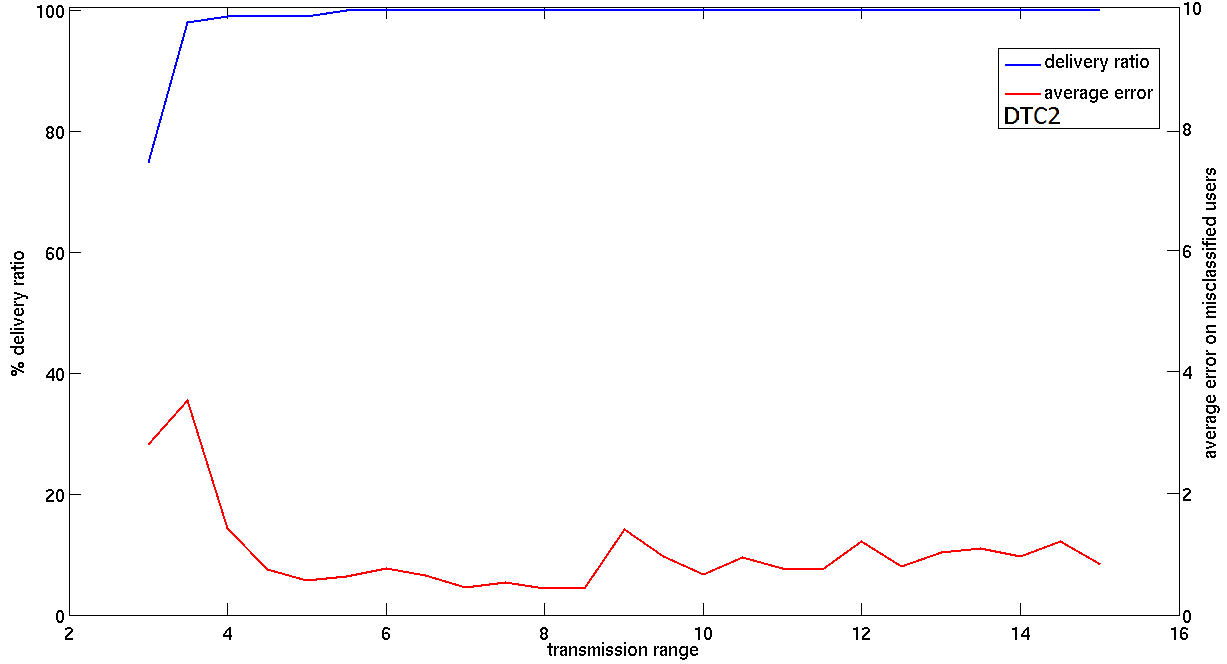
\includegraphics[scale=0.26]{figures/contribution2/error2}}
\caption{Fig.~\ref{fig:dtc2nbSends}: The percentage of forwarding users for DTC2 in comparison with the number of forwarding users for DTC. Fig.~\ref{fig:dtc2locprob}: Percentage overlap of the primary contour by the secondary contour together with the percentage reduction of the $95\%$ location probability contour of the primary transmitter in comparison with the absence of a secondary transmitter. Fig.~\ref{fig:dtc2misclass}: Percentage of misclassified users and number of receives (or updates) for DTC and DTC2. Fig.~\ref{fig:dtc2error}: The average error on the distance to footpoint for the DTC2 algorithm together with the delivery ratio.}
\end{figure*}

In this section we compare some performance metrics for simulations of the IPA algorithm with both DTC and DTC2. We look at the communication redundancy in terms of the size of the transmission range (also called communication range) and investigate whether using DTC2 has an influence on the reliability of the computation of the power of the secondary transmitter. The results are averages over three simulations. For DTC, all the users forward information and the transmission range has no influence. For DTC2, an increase in the transmission range reduces the percentage of forwarding users, as shown i Fig.~\ref{fig:dtc2nbSends}. This is because the number of forwarding neighbors per user is always maximum. However, in comparison with DTC, extra communication is needed to inform a user about the positions of his neighbors. A user needs this information to determine the forwarding set of neighbors. 

For a network with $n$ users, the number of updates for the DTC algorithm is slightly larger than $n$ because of collisions and misclassified users, as explained in section \ref{sec:dtc1}. Fig.~\ref{fig:dtc2misclass} shows the percentage of misclassified users and the number of updates in function of the kernel width. In the simulated network, the users are randomly distributed and the topology is not ideal. Therefore not all users receive their correct footpoint when using DTC2 and the number of misclassified users is slightly larger than for DTC. However, the incorrect footpoint is always received from a user within the distance of a one-hop neighbor so the error is not large. Fig.~\ref{fig:dtc2error} shows that the average error is never larger than $3\%$. It seems that as the transmission range increases, the average error also slightly increases, but this should be investigated further. When the delivery ration is smaller than one, because the transmission range is too small, the average error increases as shown in Fig.~\ref{fig:dtc2error}. 

Last, Fig.~\ref{fig:dtc2locprob} shows that using DTC2 does not have an effect on the performance of the IPA algorithm. The size of the transmission range also has no influence. We see no difference in the size of the overlap of the contours or the reduction of the location probability when using DTC or DTC2, or by varying the transmission range. We also investigated that the number of iterations for the IPA algorithm to converge lies between three and seven iterations, regardless of whether DTC or DTC2 is used.






\section{Conclusions and future work}\label{sec:conc}
We investigated the reliability of the IPA algorithm proposed by Pollin, Adams and Bahai \cite{sofie} in terms of location probability. This algorithm allows a static secondary transmitter to maximize its power without interfering with primary users. As an interference metric, the propagation contour-contour distance between the secondary and primary transmitter is used. Our simulations showed that this metric is correlated with the location probability and that the IPA algorithm makes a reliable estimation of the maximum allowed power of a secondary transmitter. 
To detect primary users and estimate the distance to the primary propagation contour, a distributed flooding algorithm, DTC, is used. To reduce the redundancy in communication, we proposed the DTC2 flooding algorithm that selects a subset of forwarding users. The algorithm reduces the number of transmissions at the cost of two things. First, we assume every user has a limited computation power available to select a subset of forwarding neighbors. However, this assumption is often valid in ad-hoc sensor networks because it is necessary for robust and scalable communication algorithms (Referentie!). Second, for a large delivery ratio DTC2 is best used in a network with a high user density. 

There are a number of options to improve our current algorithms. First, there is extensive literature on efficient flooding algorithms. Next to DTC2, we propose to investigate other cost efficient flooding algorithms and study their effect on the reliability of the IPA algorithm. Second, we want to investigate the robustness of the path loss estimation step to outliers and possibly improve this robustness. Last, the algorithm can be extended to also handle moving secondary transmitters.

\section{Acknowledgments}
The authors would like to thank Prof. Francky Catthoor and Prof. Luc De Raedt. Kurt Driessens is a post-doctoral research fellow of the Research Fund-Flanders (FWO). At the Interuniversity Micro-Electronics Center (IMEC), research on spectrum sensing is conducted in the framework of IWT SBO project ESSENCES and the EU FP7 project FARAMIR. 


% trigger a \newpage just before the given reference
% number - used to balance the columns on the last page
% adjust value as needed - may need to be readjusted if
% the document is modified later
%\IEEEtriggeratref{8}
% The "triggered" command can be changed if desired:
%\IEEEtriggercmd{\enlargethispage{-5in}}

% references section

% can use a bibliography generated by BibTeX as a .bbl file
% BibTeX documentation can be easily obtained at:
% http://www.ctan.org/tex-archive/biblio/bibtex/contrib/doc/
% The IEEEtran BibTeX style support page is at:
% http://www.michaelshell.org/tex/ieeetran/bibtex/
%\bibliographystyle{IEEEtran}
% argument is your BibTeX string definitions and bibliography database(s)
%\bibliography{IEEEabrv,../bib/paper}
%
% <OR> manually copy in the resultant .bbl file
% set second argument of \begin to the number of references
% (used to reserve space for the reference number labels box)
%\begin{thebibliography}{1}
\bibliographystyle{IEEEtran}
\bibliography{paper}
%\end{thebibliography}


\end{document}


